% Appendix C
\pagebreak
\section{Waspmote Battery Life Analysis}
\label{AppendixD} % For referencing this appendix elsewhere, use 

\subsection{Introduction: XBee and Waspmote start-up times}
\label{startup}
For the XBee node to join an existing network there are two power related possibilities. Either the Waspmote has been turned on already sufficiently long and the XBee had more than enough time to join the network, or either the XBee wasn't joined yet and the program needs to wait on this. From the experiments done at our apartment we came to following conclusions:
\begin{enumerate}
\item It takes about 2.5 seconds to join a network after powered on.
\item If the XBee is joined, the program still needs to confirm this. This takes 452 milliseconds.
\item The sending time is constant, about 158 ms, if the XBee had more than 2.5 seconds to join. However in case the XBee must send immediately after it is joined, the sending time is not constant and takes on average 611 milliseconds.
\item The sending time increases if there are more obstructions between the antennas. 
\end{enumerate}
Table \ref{tab:sendTime} sums up the results of the distance-relation test.
\begin{table}[!ht]
\begin{center}
\begin{tabular}[!ht]{|c|c|}
\hline
\textbf{Distance} & \textbf{Average sending time (ms)}\\
\hline
Air & 158\\
\hline
1 Floor & 268\\
\hline
2 Floors & 357\\
\hline
3 Floors & 484\\
\hline
4 Floors & 558\\
\hline
5 Floors & unreachable\\
\hline
\end{tabular}
\caption{Distance consequence on send times}
\label{tab:sendTime}
\end{center}
\end{table}\\
To save power the Waspmote can store the values for a user determined time. Taking samples and save them to EEPROM in case of hibernate mode takes only 6 - 7\% of the time to measure and send. Table \ref{tab:sendTime3} confirms this.



%--------------------------------------------------------------------
\subsection{High Performance Mode, without ZigBee sleep}
For this calculations it is supposed the batteries are in good condition and can be used with optimal conditions. The time values are taken from the third test scenario discussed in section \ref{second}, meaning that the Waspmote uses \textit{Hibernate} or \textit{Deepsleep} and the XBee is completely disconnected from the network.
The results are shown in figures \ref{fig:batCalcHP}, \ref{fig:batCalcHP1} and table \ref{fig:consump}.\\
%--------------------------------------------------------------------
\begin{figure}[htbp]
\centering
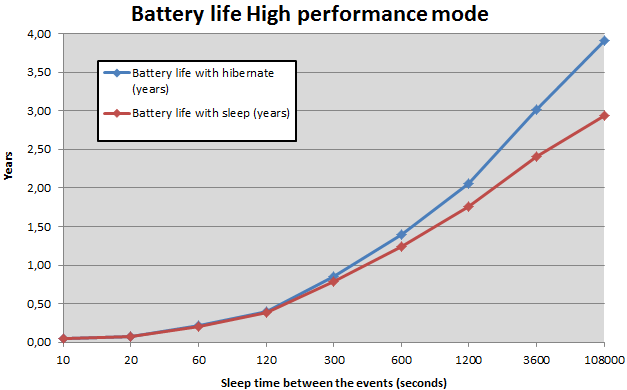
\includegraphics[height=8cm]{batCalcHP}
\caption{Battery life in High performance mode ( $\circlearrowleft$ \ref{batLife1} )}
\label{fig:batCalcHP}
\end{figure}
%-----------------------------
\begin{figure}[htbp]
\centering
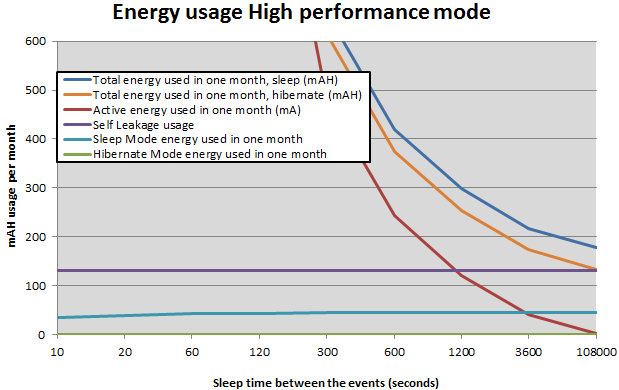
\includegraphics[height=8cm]{battery1}
\caption{Energy usage in High performance mode ( $\circlearrowleft$ \ref{batLife1} )}
\label{fig:batCalcHP1}
\end{figure}
%-----------------------------
\begin{figure}[htbp]
\centering
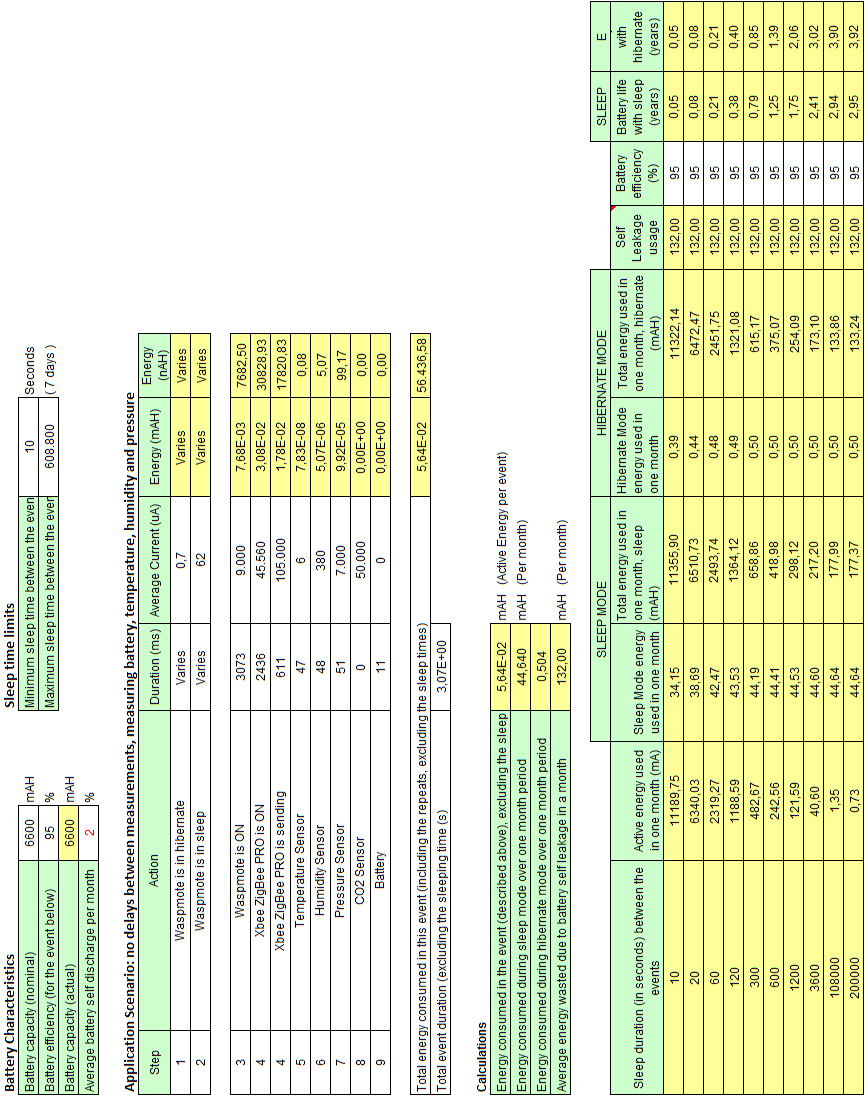
\includegraphics[height=23cm]{cons1}
\caption{Energy usage in High performance mode ( $\circlearrowleft$ \ref{batLife1} )}
\label{fig:consump}
\end{figure}\\
\vfill
\pagebreak
\noindent
The graph in figure \ref{fig:batCalcHP1} breaks down the total energy consumption to five categories. It shows the monthly energy consumption as a function of the time between the events. For small intervals the active energy usage is huge. Only from 20 minutes sleep time, the self-discharge becomes dominant and from 3 hours on the sleep mode current also becomes dominant.\\
The implementation of this mode will depend on the nodes sleep settings. For \textit{Deep Sleep} the values can simply be stored on the heap, but for \textit{Hibernate} the values must be written to EEPROM.\\
Because of the size limit of a ZigBee packet we can store maximum 30 values and send them in one packet. However, if the sensor measuring interval is small the user can opt to store more values and send two or more packets after each other. The values for Power Saver in table \ref{tab:cons2} are of an example scenario that takes 60 measurements and then sends them in two packets to the gateway. It are also those results which are put in function of time in figure \ref{fig:batCalcPS}.\\
By reducing the sensor measurement accuracy battery life can be extended with modest 3 - 4\%, best case scenario.\\
In case the measuring intervals are small it is recommended to use \textit{Deep Sleep} instead of \textit{Hibernate}, since in hibernate the values are written to EEPROM. Equation \ref{eq:1} shows this can be very destructive for the Waspmote. Depending on how much freedom the user is given, the program can make the decision to switch to \textit{Deep Sleep} on itself, or the installation's administrator can control this.
\clearpage
%-------------------------------------------------------------------
\subsection{Power Saver Mode, without ZigBee sleep}
For these calculations Power Saver Mode is supposed. The Waspmote will switch on to measure sensors but not to send the data. The values will only be sent once every 60 samples, saving energy. The results are shown in figures \ref{fig:batCalcPS}, \ref{fig:batCalcPS1} and tables \ref{tab:sendTime3} and \ref{fig:consump2}. Finally table \ref{tab:cons2} summarizes the battery duration in years of both performance and power saver mode.\\
\begin{figure}[!ht]
\centering
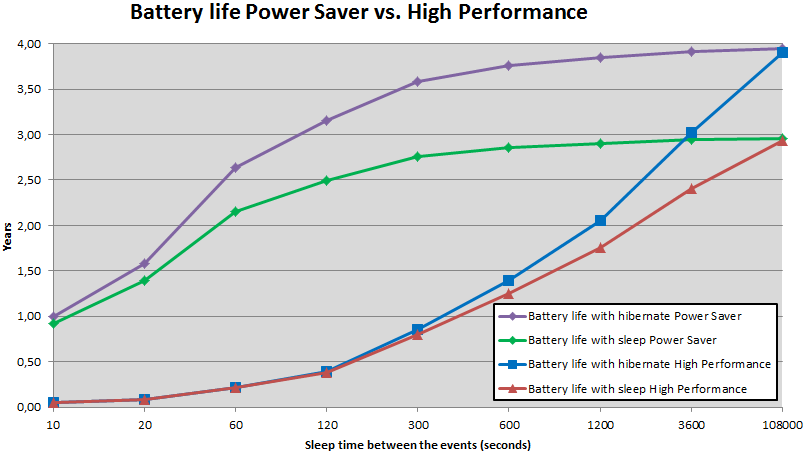
\includegraphics[height=8cm]{battery2}
%\rule{30em}{0.5pt}
\caption{Battery life High Performance vs. Power Saver $\circlearrowleft$ \ref{powerSaver} )}
\label{fig:batCalcPS}
\end{figure}
%-------------------------
\begin{figure}[htbp]
\centering
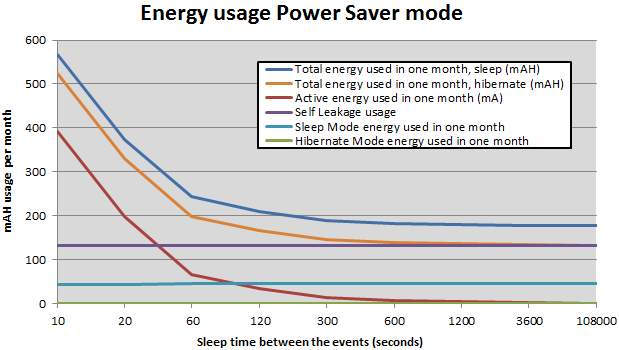
\includegraphics[height=8cm]{battery3}
\caption{Energy usage in Power Saver mode ( $\circlearrowleft$ \ref{powerSaver} )}
\label{fig:batCalcPS1}
\end{figure}
%--------------------------------
\begin{table}[!ht]
\begin{center}
\begin{tabular}{cc|c||c|c|l}
\cline{2-5}
 & \multicolumn{2}{ |c|| }{Deep Sleep} & \multicolumn{2}{c}{Hibernate}\vline\\ \cline{1-5}
\multicolumn{1}{ |c| }{Sleep duration} & High Performance & Power Saver & High Performance & Power Saver    \\ \cline{1-5}
\multicolumn{1}{ |c| }{10s} & 0,05 & 0,92 & 0,05 & 1,00    \\ %\cline{1-5}
\hline
\multicolumn{1}{ |c| }{1min} & 0,21 & 2,15 & 0,21 & 2,63   \\ %\cline{1-5}
\hline
\multicolumn{1}{ |c| }{3min} & 0,79 & 2,75 & 0,85 & 3,59   \\ %\cline{1-5}
\hline
\multicolumn{1}{ |c| }{10min} & 1,25 & 2,85 & 1,39 & 3,76   \\ %\cline{1-5}
\hline
\multicolumn{1}{ |c| }{20min} & 1,75 & 2,90 & 2,06 & 3,85  \\ %\cline{1-5}
\hline
\multicolumn{1}{ |c| }{1h} & 2,41 & 2,94 &3,02 & 3,91    \\ %\cline{1-5}
\hline
\multicolumn{1}{ |c| }{3h} & 2,94 & 2,96 &3,90 & 3,94    \\ %\cline{1-5}
\hline
%\multicolumn{1}{ |c  }{\multirow{2}{*}{Powers} } &
%\multicolumn{1}{ |c| }{gcd} & 2 & 2 & 0 & 0 & min \\ \cline{2-6}
%\multicolumn{1}{ |c  }{}                        &
%\multicolumn{1}{ |c| }{lcm} & 3 & 3 & 1 & 1 & max \\ \cline{1-6}
\end{tabular}
\caption{Battery life in years for High Performance and Power Saver}
\label{tab:cons2}
\end{center}
\end{table}
%-----------------------------
\begin{table}[!ht]
\begin{center}
\begin{tabular}[!ht]{|c|c|}
\hline
\textbf{Nr of samples per sensor} & \textbf{Average ON time (ms)}\\
\hline
10 & 210\\
\hline
3 & 194\\
\hline
\end{tabular}
\caption{Time needed to sample and store 4 sensors}
\label{tab:sendTime3}
\end{center}
\end{table}
\pagebreak
%-----------------------
\begin{figure}[htbp]
\centering
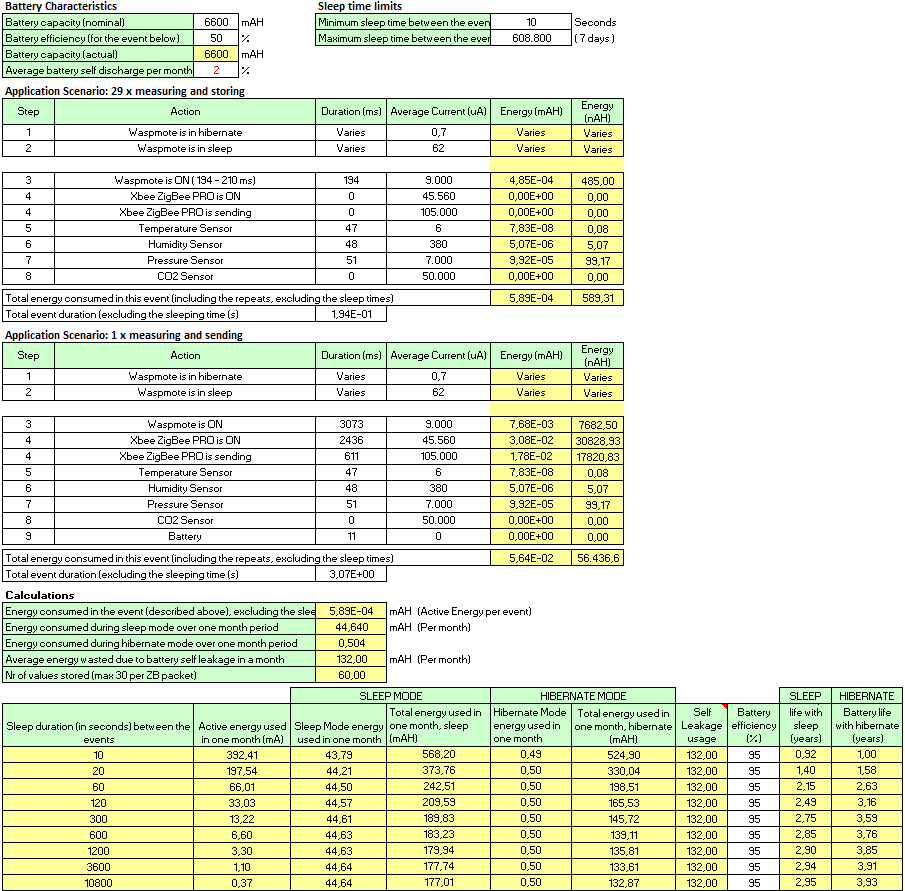
\includegraphics[height=18cm]{cons2}
\caption{Energy usage in Power Saver mode ( $\circlearrowleft$ \ref{powerSaver} )}
\label{fig:consump2}
\end{figure}
%-------------------------------------------------------------------
\clearpage
\pagebreak
